\chapter{ML-Modelle}
In dieser Arbeit wird die Device-Based Indoor-Lokalisation auf basis von Sensorwerten untersucht.
Das ist inspiriert von dem Orientierungssinn von Mensch und Tier.
Dabei werden diskrete Standorte unterschieden, sowie ob eine Anomalie entdeckt wurde,
d. h. ob das Modell sich an einem unbekannten Standort oder auf einem unbekannten Pfad befindet.
\newline
\newline
Abbildung \ref{fig:model_idea} zeigt die Architektur des verfolgten Ansatzes.
Zunächst werden aus den Sensorwerten Features extrahiert.
Die resultierende Feature-Menge wird dann von dem ML-Modell genutzt, um den Standort zu klassifizieren.
Zuletzt wird auf basis historischer Daten und dem Klassifizierungsergebnis in einem Analyseschritt (TODO: ML Ansatz?) bestimmt, ob eine Anomalie vorliegt.
Im Vergleich zu der Architektur von Mian \cite{naveedThesis} können die Klassifizierungsergebnisse bei der Feature-Extrahierung weiter verarbeitet werden.
\begin{figure}[h!]
    \centering
    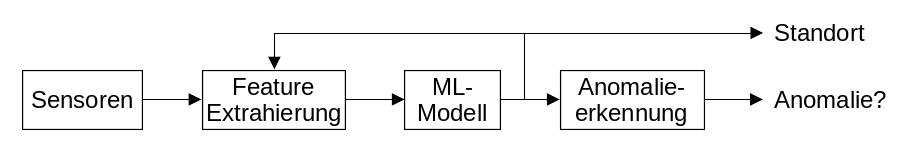
\includegraphics[width=\linewidth]{images/model_idea.png}
    \caption{Architektur des verfolgten Ansatzes.}
    \label{fig:model_idea}
\end{figure}
\newline
In dieser Arbeit Entscheidungsbaum basierte Klassifizierer mit KNN verglichen, insbesondere den von Mian verwendeten Ansatz mit FFNN.
Entscheidungsbäume sind deutlich effizienter als KNN, weswegen diese bei vergleichbarer Klassifizierungsgenauigkeit und Fehlertoleranz die preferierte Wahl sind.

\iffalse
Eigentlich eignen sich \textit{rekurrente neuronale Netze} (RNN) gut für diese Aufgabe, da serielle Daten verarbeitet werden
und zeitliche Abhängigkeiten für die Klassifizierung wichtig sind (TODO: Quelle).
Aber in dieser Arbeit wurde sich dagegen entschieden, da diese sehr rechenaufwändig sind und viel Speicher benötigen im Vergleich zu FFNN oder Entscheidungswälder,
weshalb diese suboptimal für kleine Mikrocontroller sind (TODO: Quelle).
\fi

\section{Standortenkodierung}
\begin{itemize}
    \item Was ist ein Standort? Wie ist er Definiert?
    \item Enumeriere alle 3 Optionen, sag, dass Naveed schon eine gemacht hat.
    \item Können diese Ansätze automatisch gelabelt werden? => Proximity Ansatz über mit Koordinaten festgelegten Orten
    \item Wie werden Orte modelliert?
    \item Warum wurden die Orte so modelliert?
    \item Wie werden Pfade zwischen Orten modelliert?
    \item Sollte das Modell ausgeben können, dass kein Ort erkannt wurde? => Das ist eines der Enkodierungansätze?
    \item Sollten Pfade erkannt werden können? => Eig Konsequenz aus der Evaluation, aber hier kann man davon reden, dass das Problem damit signifikant komplexer wird,
          weil nicht nur die Knoten des Graphen erkannt werden, sondern auch die Kanten
    \item Wie hilft es bei der Anomalieerkennung? => Weg verlassen
    \begin{itemize}
        \item Was ist Anomalieerkennung?
        \item Kann man ausgeben, dass eine Anomalieerkannt wurde?
        \item Vor- und Nachteile verschiedener Ansätze
        \item Nicht in ML lösen, sondern Post-Processing (Auf Evaluationskapitel verweisen)
        \item Actually: Man könnte es simulieren mit den Metriken als Features für ein Modell. KABOOF!  => Diskutiere Analyse Ansatz vs. ML-Ansatz! :D
    \end{itemize}
\end{itemize}

\section{Entscheidungswald}
\begin{itemize}
    \item Rede über Entscheidungswälder => Warum wurde ein Wald und kein Baum verwendet? Können wir uns so viele Bäume leisten? (HMM, wurd das nicht schon im Grundlagen Kapitel geklärt?)
    \item Wie wird automatisch das beste Modell gefunden?
    \item Warum trainieren wir es so => Um die beste Konfiguration zu finden unter den bestehenden Restriktionen.
    \item Welche Restriktionen werden eingefordert?
    \item Warum gibt es diese Restriktionen?
    \item Welchen Einfluss hätte es, gäbe es diese nicht?
    \item Warum wurde diese Ensemble-Methode benutzt?
\end{itemize}

\section{Feed Forward Neuronales Netzwerk}
\begin{itemize}
    \item Wie viele Hidden Layers und Neuronen sollte es haben?
    \item Welche Aktivierungsfunktionen werden verwendet?
    \item Braucht man mehr Neuronen/Hidden Layer mit steigender Ort Anzahl?
    \item OneHot Encoding der Daten => Kategorische Daten
\end{itemize}

\section{Feedback Kanten}
\begin{itemize}
    \item Was ist das?
    \item Wofür ist das Relevant?
    \item Wie funktioniert es?
    \item Wie wird das Problem umformuliert, für künstliche Rekurenz?
\end{itemize}

\section{Training der Modelle}
\begin{itemize}
    \item Trainieren in Phasen => Erklären wie es genau funktioniert?
    \item Warum trainieren wir in Phasen? => Erkläre, dass wir Klassifizierungsfehler lernen wollen, damit wir wieder zurückfinden.
    \item Sag das wir die Zyklen der einzelnen Pfade nutzen
    \item Werden mehr Trainingsdaten benötigt mit steigender Ort Anzahl? Wenn ja wie viel?
    \item Doppeltes Trainieren nach Analyse der Feature Importance.
    \item Warum machen wir das so?
    \item Zufälliges Relabeling im Training? Warum und wie funktionierts?
    \item Anteil der Daten der gerelabelt wird steigt mit Anzahl der Zyklen
\end{itemize}
